\ExplSyntaxOn
\makeatletter

\@ifclassloaded {book}
{
    \RequirePackage { geometry }
    \RequirePackage { setspace }
    \RequirePackage { epigraph }
    \RequirePackage { lineno }
    \@ifclasswith{ book } { draft } {}
        { \RequirePackage [ tracking=smallcaps, babel=true, ] { microtype } }
    \RequirePackage [final, colorlinks, allcolors=black] { hyperref }
}{}
\RequirePackage [ spanish ] { babel }
\RequirePackage { enumitem }
\RequirePackage { biblatex }
\RequirePackage { graphicx }
\RequirePackage { amsthm, mathtools }

% Set page margins
\@ifclassloaded {book}
{
    \geometry
    {
        includehead,
        paper = letterpaper,
        left = 3cm,
        right = 2cm,
        bottom = 2cm,
        top = 2cm,
        marginparsep = 10pt,
        marginparwidth = 2cm,
    }
}{}

\setlist{nosep}

% Set fonts
\usepackage{fontspec}
\usepackage[bold-style=ISO]{unicode-math}
\@ifclassloaded {book}
{
    \setmainfont{STIX Two Text}
    \setmathfont{STIX Two Math}
}
{
    \setmainfont{Source Sans Pro}
    \setsansfont{Source Sans Pro}
    \setmathfont[Scale=MatchLowercase]{STIX Two Math}
}
\newcommand{\titlefont}{\bfseries}

% Set basic spacing
\@ifclassloaded {book}
{
    \setlength { \parindent } { 8.46pt }
    \setlength { \parskip } { 6pt }
    \onehalfspacing
}{}

% Bibliography
\addbibresource{references.bib}

% Theorems
\newtheoremstyle{teo}% name
    {.5\baselineskip}% Space above
    {.5\baselineskip}% Space below
    {}% Body font
    {}% Indent amount
    {\addfontfeatures{LetterSpace=5}\scshape}% Theorem head font
    {.}% Punctuation after theorem head
    {.5em}% Space after theorem head
    {}% Theorem head spec (can be left empty, meaning ‘normal’)
\theoremstyle{teo}
\@ifclassloaded {book}
    {\numberwithin{equation}{chapter}}
    {\numberwithin{equation}{section}}
\newtheorem{defi}[equation]{Definición}
\newtheorem{lem}[equation]{Lema}
\newtheorem{teo}[equation]{Teorema}
\newtheorem{cor}[equation]{Corolario}
\newtheorem{ques}[equation]{Pregunta}

% QED symbol
\renewcommand\qedsymbol{\textsc{q.e.d.}}

% Sectioning commands
\@ifclassloaded {book}
{
    \usepackage[explicit]{titlesec}
    \titleformat
        {\chapter}
        [display]
        {\titlefont}
        {
            \centering
            \fontsize{14}{14}\selectfont
            \UpperCase{Capítulo}~\thechapter\\[10pt]
            \fontsize{12}{12}\selectfont
            \UpperCase{#1}
        }
        {0ex}
        {\centering}
    \titleformat{name=\chapter, numberless}
        [block]
        {\titlefont}
        {\fontsize{14}{14}\selectfont\UpperCase{#1}}
        {0ex}
        {\centering}
        \titleformat
        {\section}
        {\titlefont}
        {\thesection\fontsize{12}{12}\selectfont\ #1}
        {0ex}
        {}
    \titleformat{name=\section, numberless}
        [block]
        {\titlefont}
        {\fontsize{12}{12}\selectfont #1}
        {0ex}
        {}
}{}

% USB logo
\cs_new:Npn \th_print_logo_head:n #1
    {
        \group_begin:
            \centering
            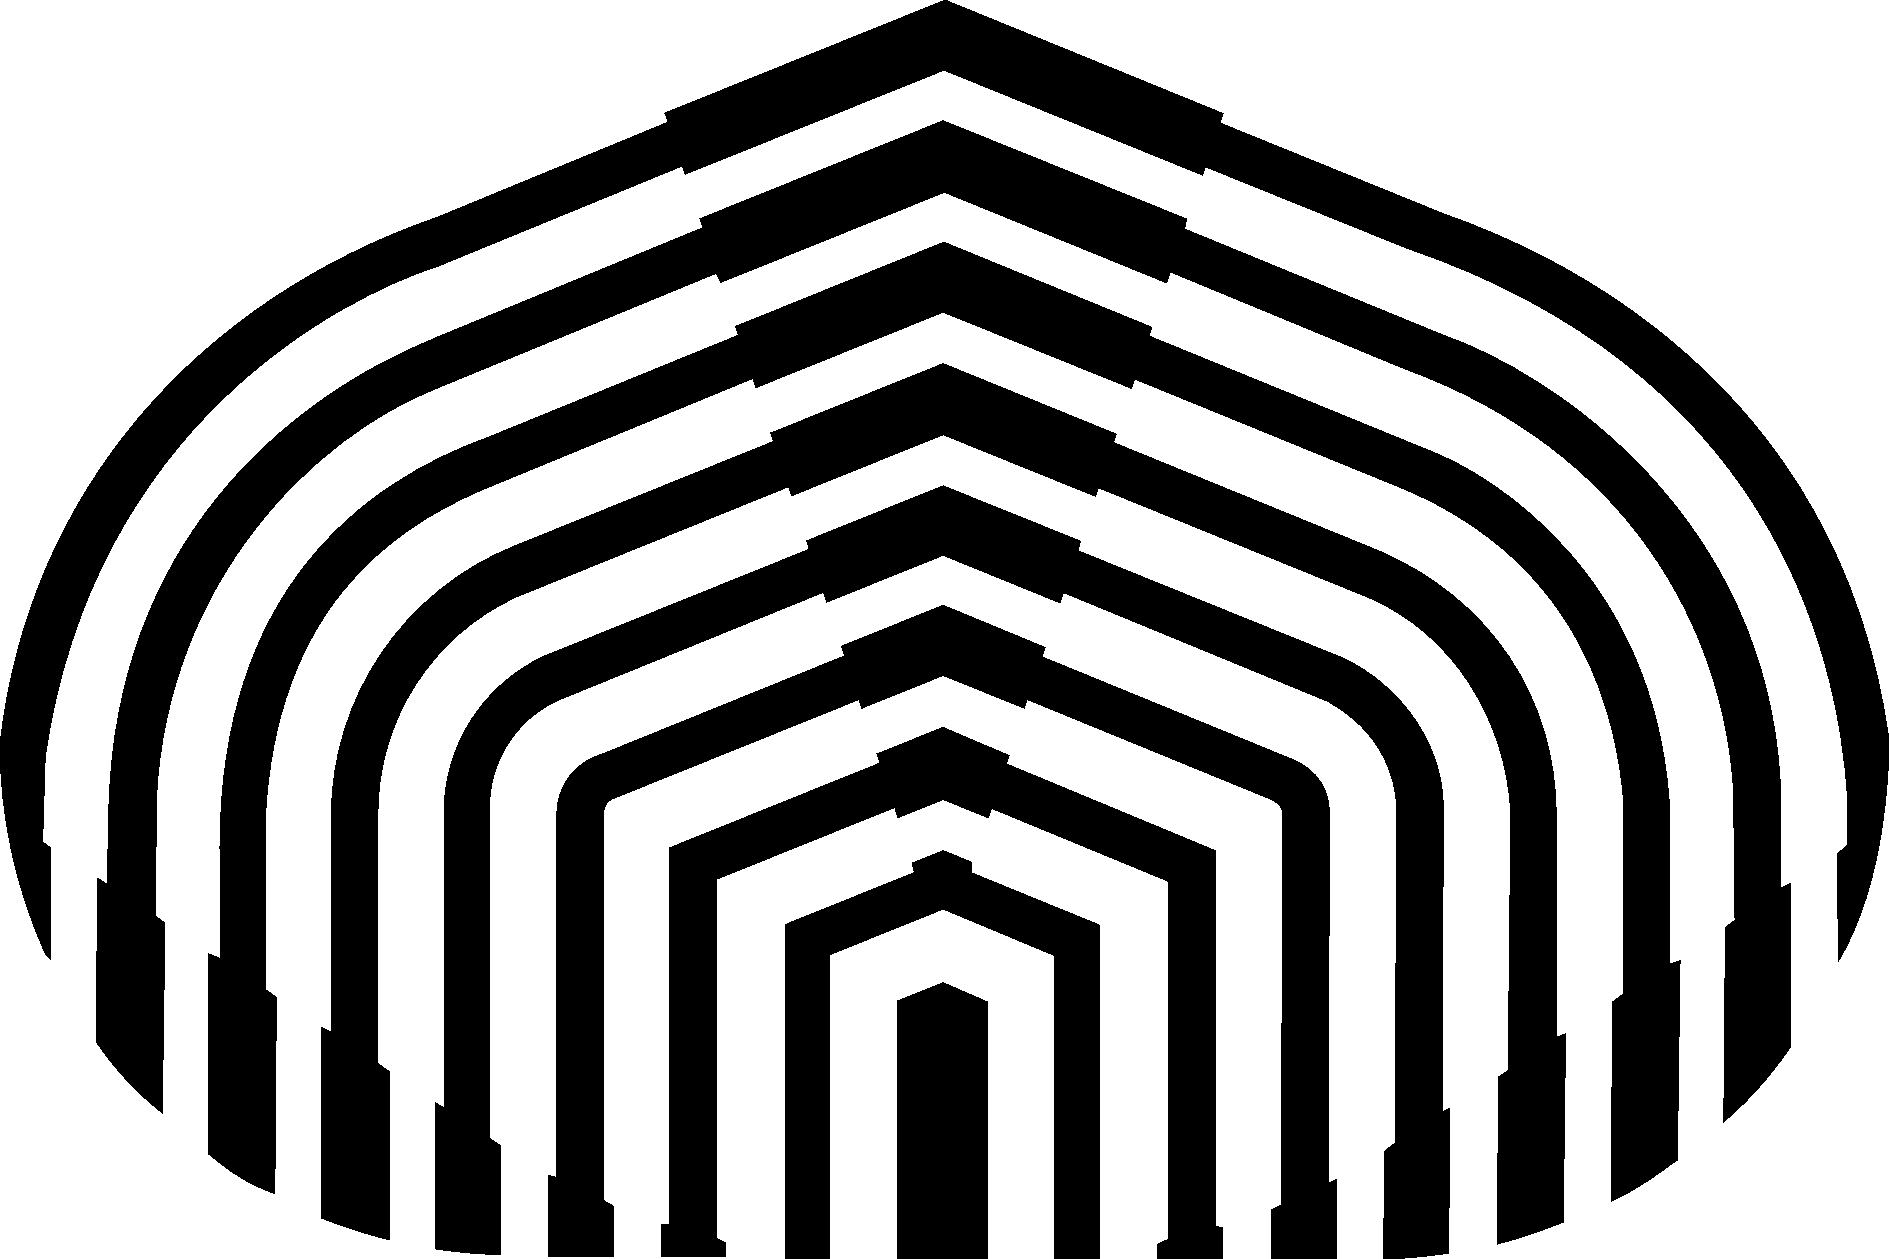
\includegraphics[scale=.3]{resources/usblogo} \\
            { \titlefont \UpperCase{#1} }
            \tex_par:D
        \group_end:
    }

\NewDocumentCommand{ \UpperCase }{ m }
    {
        \group_begin:
        \addfontfeatures{LetterSpace=10}
        \text_uppercase:n { #1 }
        \group_end:
    }

\NewDocumentCommand{ \UppercaseBold }{ m }
    {
        { \titlefont\UpperCase{#1} }
    }

\NewDocumentCommand{ \PrintUsbLogo }{ m }
    {
        \th_print_logo_head:n { #1 }
    }

\@ifclassloaded{book}
{
    \RequirePackage{tocloft}
    \setlength{\cftchapindent}{0pt}
    \setlength{\cftsecindent}{0pt}
    \NewDocumentCommand{ \ToC }{}
    {
        \clearpage
        \group_begin:
        \renewcommand{\symbf}[1]{##1}
        \linespread{1}
        \chapter*{Índice~General}
        \@starttoc{toc}
        \group_end:
    }
}{}

% Notes
\@ifclassloaded {book}
{
    \reversemarginpar
    \NewDocumentCommand{ \note }{ m }
    {
        \@ifclasswith{ book } { draft }
        {
            \begingroup
            \ttfamily
            \footnotesize
            \textlangle #1 \textrangle
            \endgroup
        } {}
        \PackageWarning{Notes}{Revisar~nota}
    }
}{}

% Wrapping
\newlength{\wrapwd}
\NewDocumentCommand { \wrapto } { o o m }
{
    \IfNoValueTF { #1 }
        { \setlength{\wrapwd}{.6\linewidth} }
        { \setlength{\wrapwd}{#1} }
    \IfNoValueTF { #2 }
        { \let\wrapal\raggedright }
        { \let\wrapal#2 }
    \begin{minipage}{\wrapwd}
        \wrapal
        #3
    \end{minipage}
}

% Conditionals
\newif \ifcaratula
\newif \ifpaginatitulo
\newif \ifresumen
\newif \ifagradecimientos
\newif \iflistas
\newif \iftoc
\newif \ifintro
\newif \ifbasicos
\newif \ifmainproofs
\newif \ifreferencias

% macros
\newcommand { \MainTitle }
    {
        Estudio~comparativo~de~tres~demostraciones~
        del~teorema~de~inconsistencia~de~Kunen.
    }

\newcommand {\shorttitle} {El~teorema~de~inconsistencia~de~Kunen.}

\newcommand { \autor }
    {
        Jhonny~Alexander~Lanzuisi~Berrizbeitia
    }
\newcommand {\shortname} {Jhonny~Lanzuisi}

\newcommand { \tutor }
    {
        Jesús~Nieto~Martínez
    }

\newcommand { \coord }
    {
        Matemáticas
    }

\NewDocumentCommand { \StrIfEq } { m m m m }
    {
        \str_if_eq:nnTF { #1 } { #2 } { #3 } { #4 }
    }

\@ifclasswith{ book } { draft } { \linenumbers } {}

\ExplSyntaxOff
\makeatother

\AddToHook{begindocument}{
\let\oldalpha\alpha
\def\alpha{{\symup\oldalpha}}
\let\oldbeta\beta
\def\beta{{\symup\oldbeta}}
\let\oldgamma\gamma
\def\gamma{{\symup\oldgamma}}
\let\olddelta\delta
\def\delta{{\symup\olddelta}}
\let\oldepsilon\epsilon
\def\epsilon{{\symup\oldepsilon}}
\let\oldzeta\zeta
\def\zeta{{\symup\oldzeta}}
\let\oldeta\eta
\def\eta{{\symup\oldeta}}
\let\oldtheta\theta
\def\theta{{\symup\oldtheta}}
\let\oldiota\iota
\def\iota{{\symup\oldiota}}
\let\oldkappa\kappa
\def\kappa{{\symup\oldkappa}}
\let\oldlambda\lambda
\def\lambda{{\symup\oldlambda}}
\let\oldmu\mu
\def\mu{{\symup\oldmu}}
\let\oldnu\nu
\def\nu{{\symup\oldnu}}
\let\oldxi\xi
\def\xi{{\symup\oldxi}}
\let\oldomicron\omicron
\def\omicron{{\symup\oldomicron}}
\let\oldpi\pi
\def\pi{{\symup\oldpi}}
\let\oldrho\rho
\def\rho{{\symup\oldrho}}
\let\oldsigma\sigma
\def\sigma{{\symup\oldsigma}}
\let\oldtau\tau
\def\tau{{\symup\oldtau}}
\let\oldupsilon\upsilon
\def\upsilon{{\symup\oldupsilon}}
\let\oldphi\phi
\def\phi{{\symup\oldphi}}
\let\oldchi\chi
\def\chi{{\symup\oldchi}}
\let\oldpsi\psi
\def\psi{{\symup\oldpsi}}
\let\oldomega\omega
\def\omega{{\symup\oldomega}}
}

\DeclareMathOperator*{\dint}{\bigtriangleup}
\DeclareMathOperator*{\cf}{cf}
\DeclareMathOperator{\Con}{Con}
\DeclareMathOperator{\Crit}{crit}
\DeclareMathOperator{\rank}{rank}
\DeclareMathOperator{\ran}{ran}
\DeclareMathOperator{\Eu}{E_U}
\DeclareMathOperator{\Ult}{Ult}
\DeclareMathOperator{\tc}{tc}
\DeclareMathOperator{\ot}{ot}

\newcommand\model[1]{\mathfrak { #1 }}
\newcommand\set[1]{\left\{ #1 \right\}}
\newcommand\lex[1]{\mathcal { #1 }}
\newcommand\crit[1]{\Crit (#1)}
\makeatletter
\newcommand\pwset[2][]
{
    \ifnum\pdf@strcmp{\detokenize{#1}}{}=0\relax
        \mathcal{P}(#2)
    \else
        \mathcal{P}\kern-2pt_{#1}(#2)
    \fi
}
\makeatother
\newcommand\concept[1]{#1}
\newcommand\op[1]{\langle #1 \rangle}
\newcommand\seq[1]{\langle #1 \rangle}
\newcommand\con[1]{\Con ( #1 )}
\newcommand\embed{\prec}
\newcommand\lst{\lex{L}_\in}
\newcommand\cna[1]{\StrIfEq{#1}{.}{c.\,n.\,a.}{c.\,n.\,a.#1}}
\newcommand\ecl[1]{{(#1)}_U^0}
\newcommand{\id}{\symup{id}}
\newcommand{\rest}{\kern1.5pt\vert\kern1.5pt}
\newcommand{\ChapterNoNumber}[1]
{
    \chapter*{#1}
    \addcontentsline{toc}{chapter}{\protect\numberline{} #1}%
}

\ifdefined\initex
    \dump
\fi
